\aufgabenstellung{Mod­i­fizieren Sie das Pro­gramm, so daß es nicht Worte 
son­dern a) Buch­staben 
bzw. b) Buch­staben­paare zählt. Vergle­ichen Sie deren Häufigkeitsverteilung 
sowohl zweier in der gle­ichen Sprache ver­fassten Texte als auch zweier in 
ver­schiede­nen Sprachen abge­fasster Texte. (2 Punk­te)}




\loesung{}
Vergleicht man die Erscheinungshäufigkeit der Buchstaben in der deutschen Fassung von Kafkas Verwandlung mit der der englischen Fassung (Abb. \ref{chars}), so fällt vor allem auf, dass in beiden Sprachen der Buchstabe e am häufigsten vorkommt, wenngleich im deutschen Text mit 13,58 \% ein wenig öfter als im englischen (9,98 \%).
\begin{figure}[ht]
\begin{center}
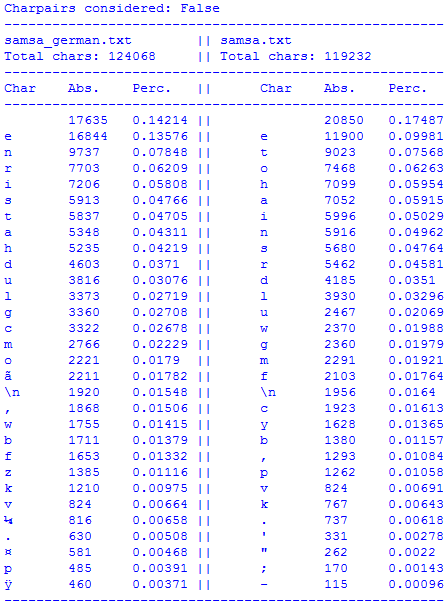
\includegraphics[width=0.8\textwidth]{img/chars}
\caption{Liste der 30 am häufigsten vorkommenden Buchstaben in Die Verwandlung (deutsch und englisch)}
\label{chars}
\end{center}
\end{figure}

Richtet man den Blick nun auf die Buchstabenpaare, so finden sich in beiden Sprachen die Paare \textit{ll} und \textit{ss} jeweils recht weit oben in den jeweiligen Listen (Abb. \ref{charpairs}). Bei anderen Paaren, wie z. B. \textit{ee} oder \textit{nn} finden sich dagegen deutliche Unterschiede in den auftretenden Häufigkeiten (40 zu 393 bzw. 389 zu 33).
\begin{figure}[ht]
\begin{center}
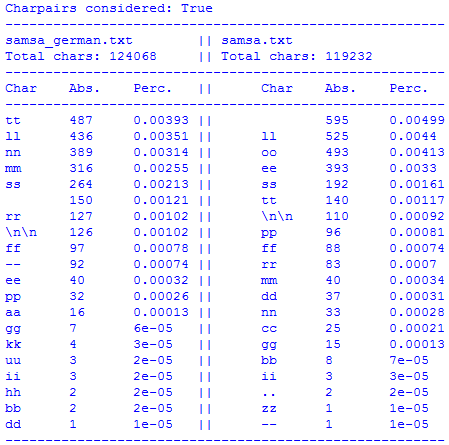
\includegraphics[width=0.8\textwidth]{img/charpairs}
\caption{Liste der 30 am häufigsten vorkommenden Buchstabenpaare in Die Verwandlung (deutsch und englisch)}
\label{charpairs}
\end{center}
\end{figure}

Bei der Häufigkeitsverteilung der Buchstaben sowie der Buchstabenpaare lässt sich in den logarithmierten Abbildungen \ref{fig:frankensteinCharpairs} bis \ref{fig:frankensteinChars} ebenfalls eine fallende Gerade erkennen, was auf eine Befolgung des Zipfschen Gesetzes hindeutet.\\




\logPlotOf{aufg04/frankenstein_pairs.csv}{Die Häufigkeit (y-Achse) der 30 
häufigsten Buchstabenpaare in Frankenstein (logarithmiert)}{fig:frankensteinCharpairs}
\logPlotOf{aufg04/samsa_pairs.csv}{Die Häufigkeit (y-Achse) der 30 
häufigsten Buchstabenpaare in Die Verwandlung (englisch) (logarithmiert)}{fig:verwandlungEnglischCharpairs}
\logPlotOf{aufg04/samsa_german_pairs.csv}{Die Häufigkeit (y-Achse) der 30 
häufigsten Buchstabenpaare in Die Verwandlung (deutsch) (logarithmiert)}{fig:verwandlungDeutschCharpairs}
\logPlotOf{aufg04/samsa.txt.csv}{Die Häufigkeit (y-Achse) der 30 
häufigsten Buchstaben in Die Verwandlung (englisch) (logarithmiert)}{fig:verwandlungEnglischChars}
\logPlotOf{aufg04/samsa_german.txt.csv}{Die Häufigkeit (y-Achse) der 30 
häufigsten Buchstabenpaare in Die Verwandlung (deutsch) (logarithmiert)}{fig:verwandlungDeutschChars}
\logPlotOf{aufg04/frankenstein.txt.csv}{Die Häufigkeit (y-Achse) der 30 
häufigsten Buchstaben in Frankenstein (logarithmiert)}{fig:frankensteinChars}